%# -*- coding: utf-8-unix -*-
% !TEX program = xelatex
% !TEX root = ../thesis.tex
% !TEX encoding = UTF-8 Unicode
%%==================================================
%% chapter02.tex for SJTU Master Thesis
%% based on CASthesis
%% modified by wei.jianwen@gmail.com
%% Encoding: UTF-8
%%==================================================

\chapter{Influences of key nodes on competition}
\label{chap5}
In this chapter, it is investigated which nodes have the most important influence for keeping or changing their orientation on a two-layer network. There exist many methods to select key nodes, such as Pagerank, degree centrality, eigenvector centrality, betweenness centrality, and closeness centrality. Moreover, in \parencite{mesgari2015, huang2014}, it has been proved that multiple indicators that use the rank difference of several node centralities are useful to identify key nodes and prevent the slow way to identify critical nodes. Based on these methods, such as single-node centrality(single indicators) and combined node centrality(multiple indicators), it is researched which method is the most effective and the most influential for selecting key nodes.  

\section{Method for selecting key nodes}
\label{sec:method for finding key nodes}
As the initial conditions for selecting key nodes, each layer consists of a \textit{BA} network with $512$ nodes, $K=3$, and $1$ external edge. Each simulation takes $100$ steps for opinion evolution, and $100$ simulations are considered for average results. In order to demonstrate the influence of key nodes, the parameters such as $p$ and $v$ are set to be the opposite consensus state to the initial state of a layer for identifying key nodes. The parameters can be set up differently on each network because each network has different critical points for the transition of the state. And then the stubborn nodes, which do not change their states during the evolution of opinion, are selected by using methods for selecting key nodes, and then the ratio of stubborn nodes is increased until the state of a network is changed into the same consensus state with the initial state of the layer for identifying key nodes. Under these conditions, the most powerful method is the fastest method to reach the same consensus state with the initial state of a layer for selecting key nodes. For example, for selecting key nodes on layer A(positive opinion), the parameters are set to be a negative consensus state. Then, as the stubborn nodes on layer A are selected by node centrality or other methods, and the ratio of the stubborn nodes is increased, a state of the network is gradually changed into a positive state. Inversely for selecting key nodes on layer B(negative opinion), the parameters are set to be a positive consensus state. Then, as the stubborn nodes on layer B are selected by the method for recognizing key nodes, and the ratio of stubborn nodes is increased, a state of the network is gradually changed into a negative state. Here, we find the fastest and most powerful method.

As the method to select stubborn nodes, we use two kinds of indicators, single indicators, and multiple indicators. As single indicators, node centralities are applied, such as Pagerank, degree, eigenvector, closeness, and betweenness. As multiple indicators, combined node centralities that consist of several node centralities are applied.
  
First, here is the way to select key nodes by using a single node centrality.
\begin{enumerate}
	\item All nodes are ranked by five node centralities(Pagerank, degree, eigenvector, closeness, betweenness).
	\item The nodes are deactivated from high ranked order until the state of network has a significant difference, i.e., the stubborn nodes are selected according to high ranked order, and the ratio of stubborn nodes is increased. 
	\item The results are compared according to node centralities. When a node centrality makes the state of network reach the fastest to the opposite consensus state with the initial condition or have the most significant change, it is the most powerful method for selecting key nodes.
	\item As the ratio of stubborn nodes is increased, the summation of $AS$, which represents the `Average States' of a network, is calculated on every single indicator. It is recognized that the larger the $AS$ value is on layer A, the more influential that indicator is, inversely the smaller the $AS$ value is on layer B, the more influential that indicator is.
\end{enumerate}

Furthermore, we research the way to recognize critical nodes by using multiple indicators such as combined node centralities(\textit{PR+DE, PR+BE, DE+BE, PR+DE+BE}). Combined node centralities are made up of several selected node centralities. When it is proven that a node centrality is useful for selecting key nodes through the simulations, the node centrality is selected as a factor of combined node centrality. Here, $2$ or $3$ node centralities are selected, such as Pagerank, degree, and betweenness. The way to recognize key nodes by using combined node centrality follows like this steps. 

\begin{enumerate}
	\item Each selected node centrality ranks all nodes. All nodes have the ranks as the number of selected node centralities.  
	\item Combined node centrality is calculated by the summation of all ranks which a node has. 
	\item All nodes are ranked again by combined node centrality. The smaller the combined node centrality is, the higher a node is ranked.        
	\item The nodes are deactivated from high ranked order until the state of network has a significant difference, i.e., the stubborn nodes are selected according to high ranked order, and the ratio of stubborn nodes is increased. 
\end{enumerate}

It has been already proven that a single node centrality has good performance to identify key nodes.\parencite{koschutzki2008, francisco2018, bianconi2018}. However, identifying key nodes by multiple indicators is still an open problem because there are lots of ways to set up and optimize the weight of each node centrality.\parencite{huang2014}  Here, we simplify the method by setting the weights as equal and calculate the summation of ranks. Although our multiple indicators need to be researched further, the multiple indicators are evaluated and compared with single indicators. The way for measuring and evaluating key nodes on the \textit{BA-BA} network are described as subsection \ref{layerA} and subsection \ref{layerB}.\\
 
\subsection{Key nodes on layer A}
\label{layerA}
\begin{figure}[!htb]
	\centering
	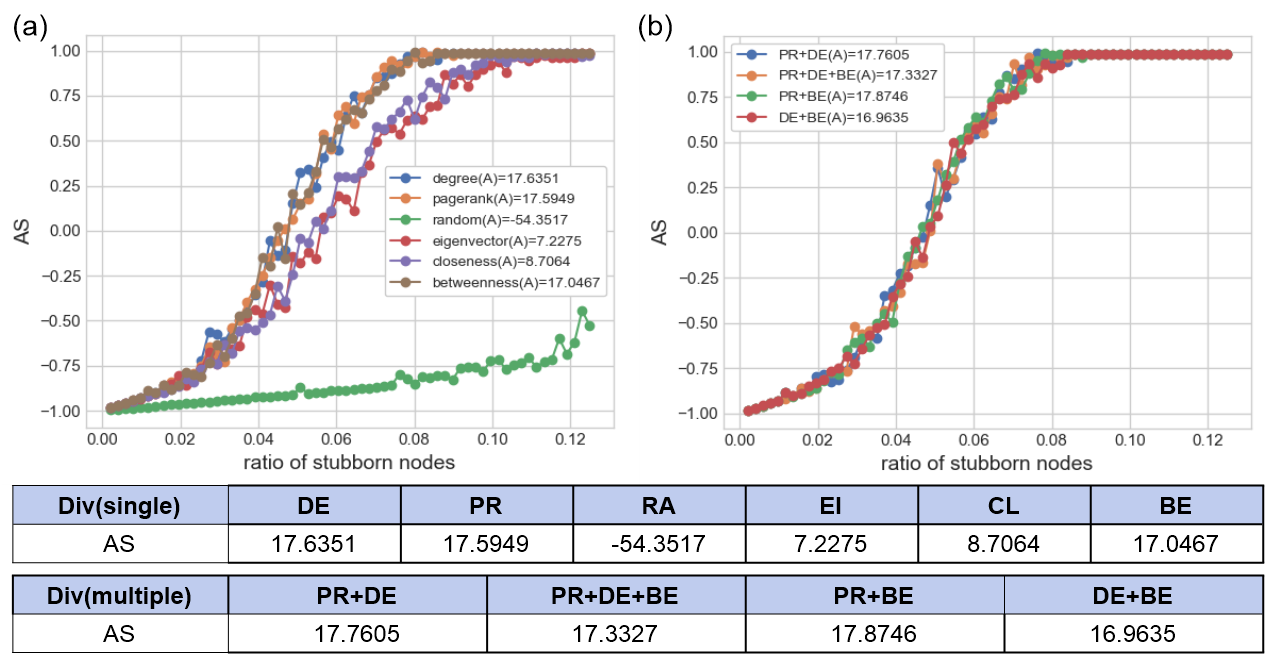
\includegraphics[width=\hsize]{figure/chap5_keynode_A.png}
	\caption{Key nodes on layer A in \textit{BA(3)-BA(3)} network($p=0.2, v=0.4$)}
	\label{chap5_keynode_A}
\end{figure}
To select key nodes on layer A, two parameters are set to be negative consensus state like $p=0.2, v=0.4$. When the parameters($p, v$) are set up for recognizing key nodes by using stubborn nodes, several things have to be considered. First, to effectively demonstrate the influence of key nodes and show the transition of the state, the parameters have to make the opposite consensus with the initial state of the selected layer. Second, parameters have to be set up close to critical points to make the transition easier. If the parameters are far from the critical points, key nodes(stubborn nodes) cannot make the state of a network changed. That makes it hard to compare the simulation results. Third, the parameters have to be set up on each network individually because each network has different critical points.  In this work, the parameters on each network are shown with simulation results and figures.   

As single indicators, five node centralities(Pagerank, degree, eigenvector, closeness, betweenness) are used, and the influence of randomly selected nodes is also compared with five node centralities. As multiple indicators, $2$ or $3$ node centralities are combined, such as Pagerank, degree, and betweenness, which have good performance as single indicators. In combined node centralities, we denote Pagerank, degree, and betweenness as \textit{PR, DE, BE}. Moreover, when they are combined, the methods are denoted as \textit{PR+DE, PR+BE, DE+BE, PR+DE+BE} by using \textit{+}. 

Fig.~\ref{chap5_keynode_A} shows the simulation result for recognizing key nodes on layer A. As a single indicator, Pagerank has the best performance. The next ranks are degree and betweenness. As multiple indicators, \textit{PR+BE} has the most effective result. The next is \textit{PR+DE}. These two methods of multiple indicators work better than Pagerank. Compared with all methods, the best method is \textit{PR+BE}. It can be found out that some multiple indicators are more useful for selecting key nodes than single indicators. \\

\subsection{Key nodes on layer B}
\label{layerB}
\begin{figure}[!htb]
	\centering
	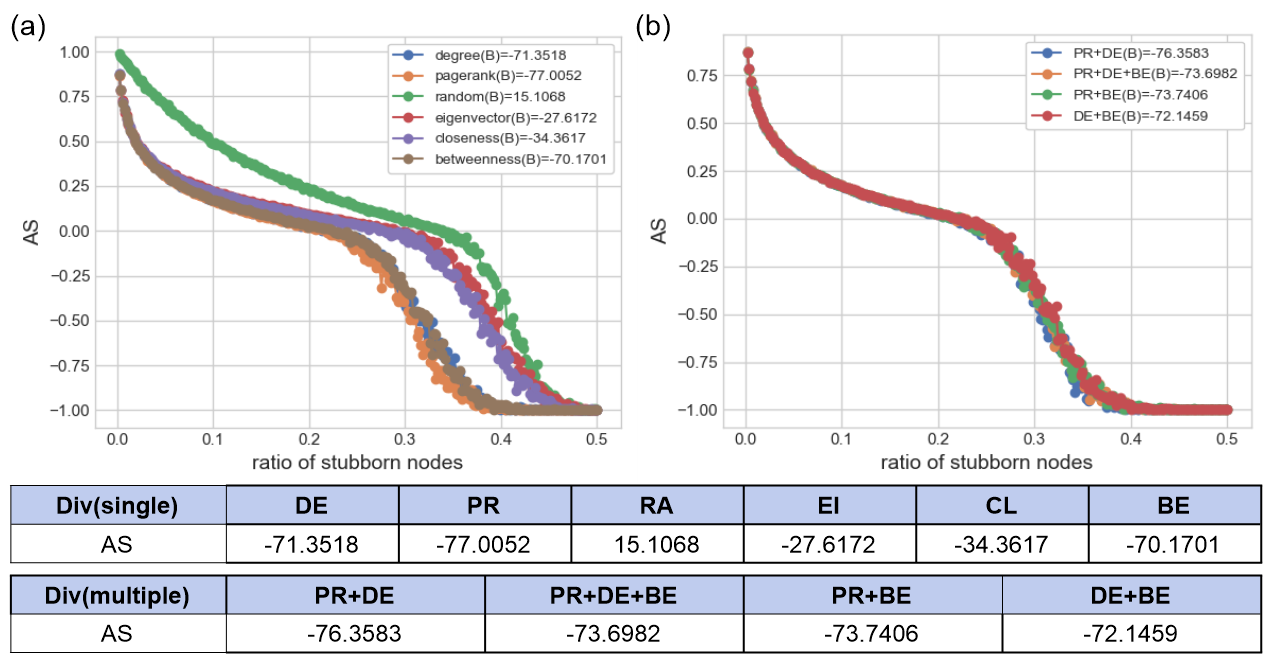
\includegraphics[width=\hsize]{figure/chap5_keynode_B.png}
	\caption{Key nodes on layer B in \textit{BA(3)-BA(3)} network($p=0.3, v=0.5$)}
	\label{chap5_keynode_B}
\end{figure}

To select key nodes on layer B, parameters are set to be positive consensus state such as $p=0.3, v=0.5$. Fig.~\ref{chap5_keynode_B} shows the simulation result for identifying key nodes on layer B. As a single indicator, the most effective way to recognize important nodes is Pagerank centrality. The next ranks are degree and betweenness. As multiple indicators, \textit{PR+DE} has the best performance. Pagerank is the most effective method for selecting key nodes on layer B. But, all multiple indicators work better than degree centrality, the second rank in single indicators. It can be found out that combined node centralities also have a good performance for selecting key nodes, though they are not the best. \\

\section{Key nodes on two-layer networks with different structures}
In this section, we select the key nodes in the networks with various structures that are described in chapter~\ref{chap3}. Node centralities and combined node centralities are also used as the methods for selecting key nodes. First, \textit{Hierarchical Model} is applied to identify critical nodes. Second, we consider the case that each layer has a different network type, such as \textit{BA-RR} or \textit{RR-BA} networks. Third, the case is considered that each layer has a different number of internal edges. Layer A can have more internal links, or layer B can have more internal links. Both cases are simulated. \\

\subsection{Key nodes in Hierarchical Model}
\begin{figure}[!htb]
	\centering
	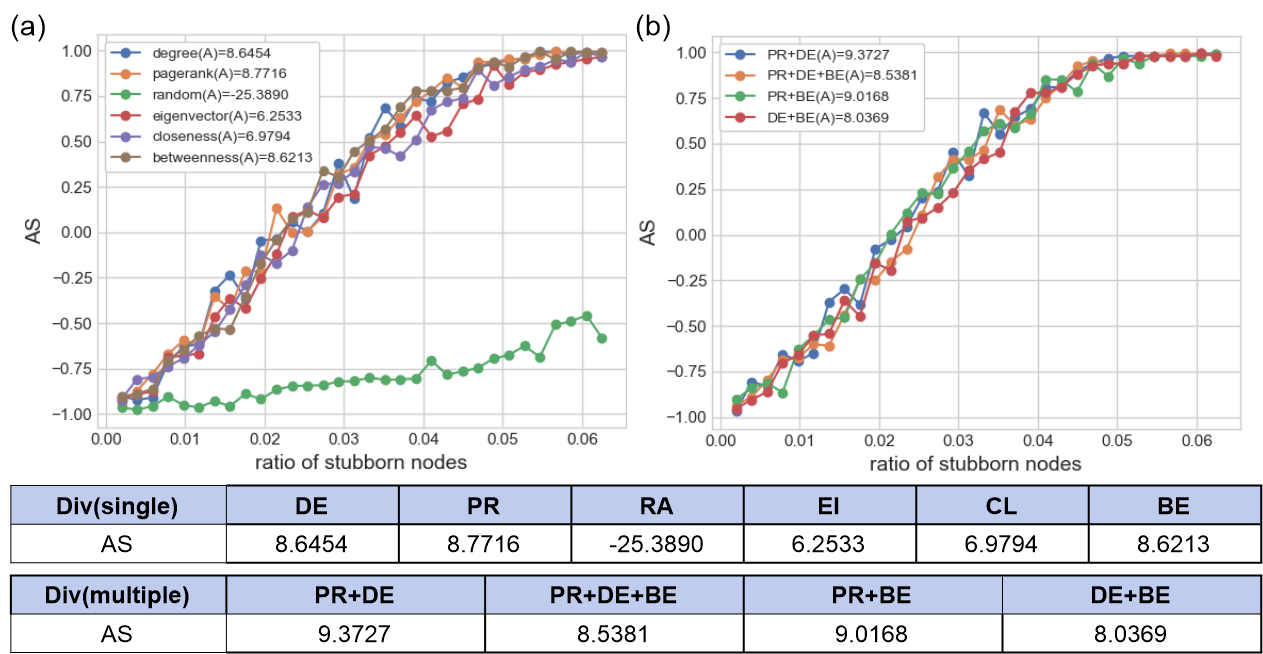
\includegraphics[width=\hsize]{figure/chap5_keynode_HM_A.png}
	\caption{Key nodes on layer A in \textit{Hierarchical Model(8)}($p=0.2, v=0.2$)}
	\label{chap5_keynode_HM_A}
\end{figure}
\begin{figure}[!htb]
	\centering
	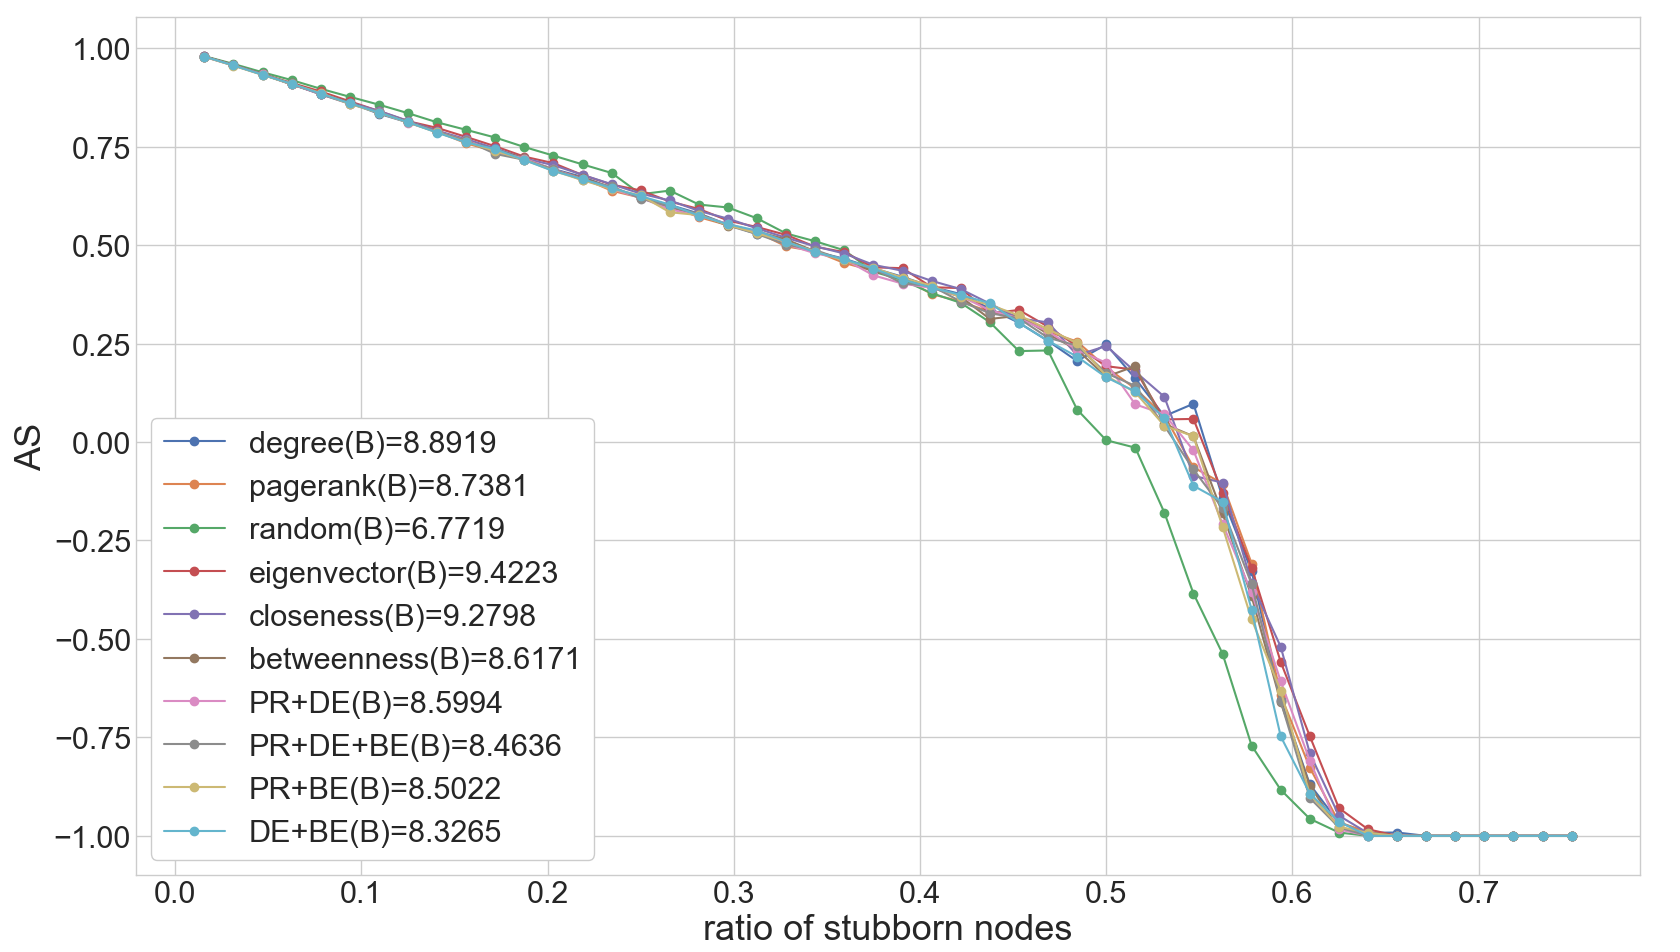
\includegraphics[width=\hsize]{figure/chap5_keynode_HM_B.png}
	\caption{Key nodes on layer B in \textit{Hierarchical Model(8)}($p=0.25, v=0.3$)}
	\label{chap5_keynode_HM_B}
\end{figure}

As described in chapter~\ref{chap3}, \textit{Hierarchical Model} is the two-layer network that the number of nodes in layer B is reduced at a specific rate, and the external links from nodes in layer B are increased accordingly. Here, each layer consists of a \textit{BA} network with $k=3$. Layer A has $512$ nodes, and layer B has $64$ nodes. We denote this model as \textit{HM(8) with BA(3)}.

Fig.~\ref{chap5_keynode_HM_A} shows the simulation result of key nodes on layer A. Simulation result represents that \textit{PR+DE} is the best method for recognizing key nodes on \textit{HM(8) with BA(3)}. The next ranks are \textit{PR+BE} and Pagerank. The curve of changing the network states shown in Fig.~\ref{chap5_keynode_HM_A} is more straight than Fig.~\ref{chap5_keynode_A}. That means the speed of changing network states(consensus time) is much faster. 

Fig.~\ref{chap5_keynode_HM_B} shows the simulation result of key nodes on layer B. However, the result is different from other simulation results. The best performance method is a random method. That means node centralities do not work on this model. Furthermore, the curve of changing the network states shown in Fig.~\ref{chap5_keynode_HM_B} is also more straight than Fig.~\ref{chap5_keynode_B}, which means the consensus is much easier, and the consensus time is much shorter. It is found out that the \textit{Hierarchical Model} produces that the indexes for key nodes are hard to recognize key nodes on layer B. Furthermore, the \textit{Hierarchical Model} is easy to reach a consensus of two-layer by key nodes. \\

\subsection{Key nodes on the two-layer network with different network types}
Here, we consider two types of networks, \textit{BA-RR} and \textit{RR-BA}. The number of internal links on each layer is set up as the same or almost the same number to exclude the influence of internal degrees. These models are compared with the \textit{BA-BA} to find out the influence of network types under the same conditions, such as $p$, $v$, and $the ratio of stubborn nodes$.  

\begin{figure}[!htb]
	\centering
	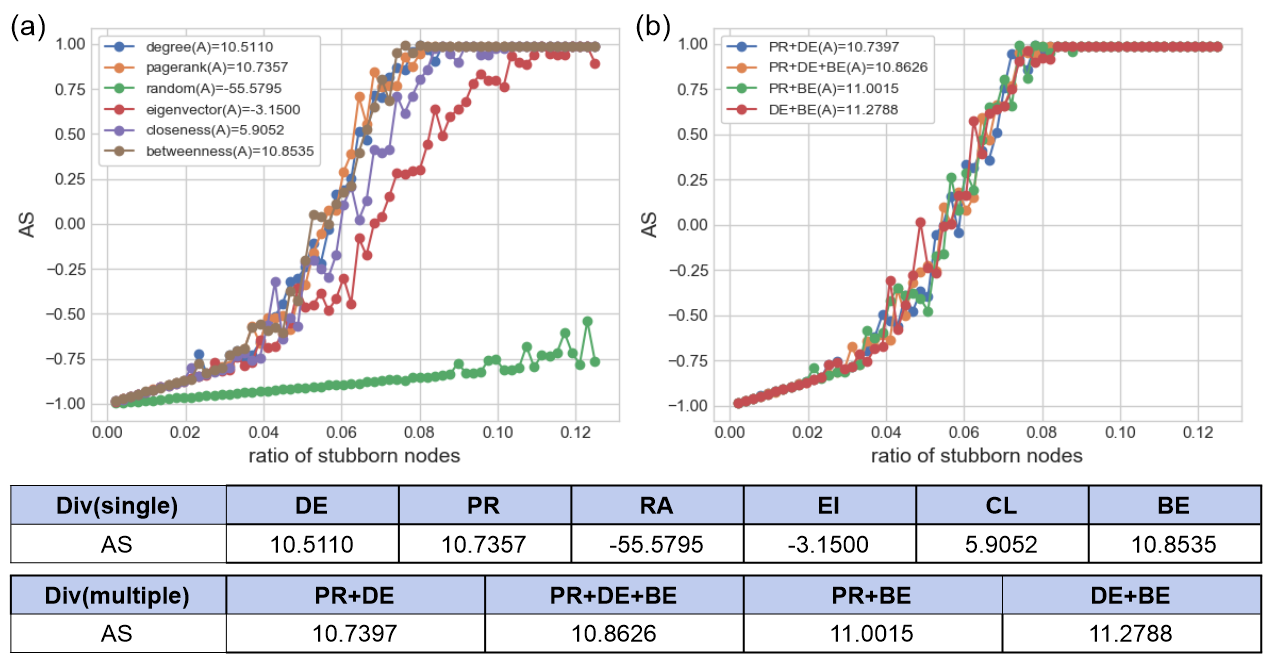
\includegraphics[width=\hsize]{figure/chap5_keynode_BA_RR_A.png}
	\caption{Key nodes on layer A in \textit{BA(3)-RR(6)} network($p=0.2, v=0.4$)}
	\label{chap5_keynode_BA_RR_A}
\end{figure}
\begin{figure}[!htb]
	\centering
	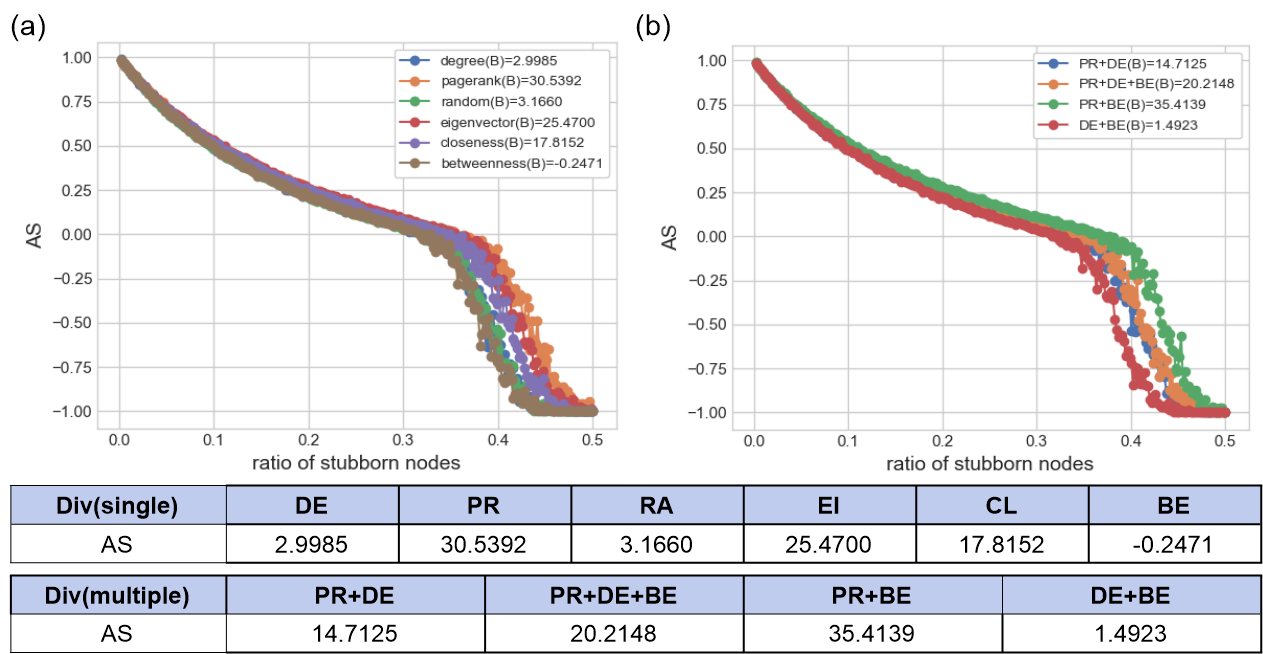
\includegraphics[width=\hsize]{figure/chap5_keynode_BA_RR_B.png}
	\caption{Key nodes on layer B in \textit{BA(3)-RR(6)} network($p=0.3, v=0.5$)}
	\label{chap5_keynode_BA_RR_B}
\end{figure}

First, the \textit{BA-RR} network is investigated. Fig.~\ref{chap5_keynode_BA_RR_A} shows the simulation result of key nodes on layer A.\textit{PR+BE} is the most powerful method. The next rank is Pagerank as a single indicator. Compared with the \textit{BA(3)-BA(3)} shown in Fig.~\ref{chap5_keynode_A}, \textit{BA(3)-RR(6)} has smaller \textit{AS} values and a more gentle curve to change the state of the network. 

Fig.~\ref{chap5_keynode_BA_RR_B} shows the simulation result of key nodes on layer B. Betweenness is the best method for identifying key nodes on layer B in the \textit{BA-RR} network. In this model, the degree centrality is not an exact method for the selection of key nodes because the degree of each node is the same in the \textit{RR} network. However, random and degree method is the third and fourth method for recognizing key nodes. That means other methods except for betweenness do not work for identifying key nodes. Compared with the \textit{BA(3)-BA(3)} shown in Fig.~\ref{chap5_keynode_B}, the \textit{BA(3)-RR(6)} has more massive \textit{AS} values and a more gentle curve to change the state of the network. 

\begin{figure}[!htb]
	\centering
	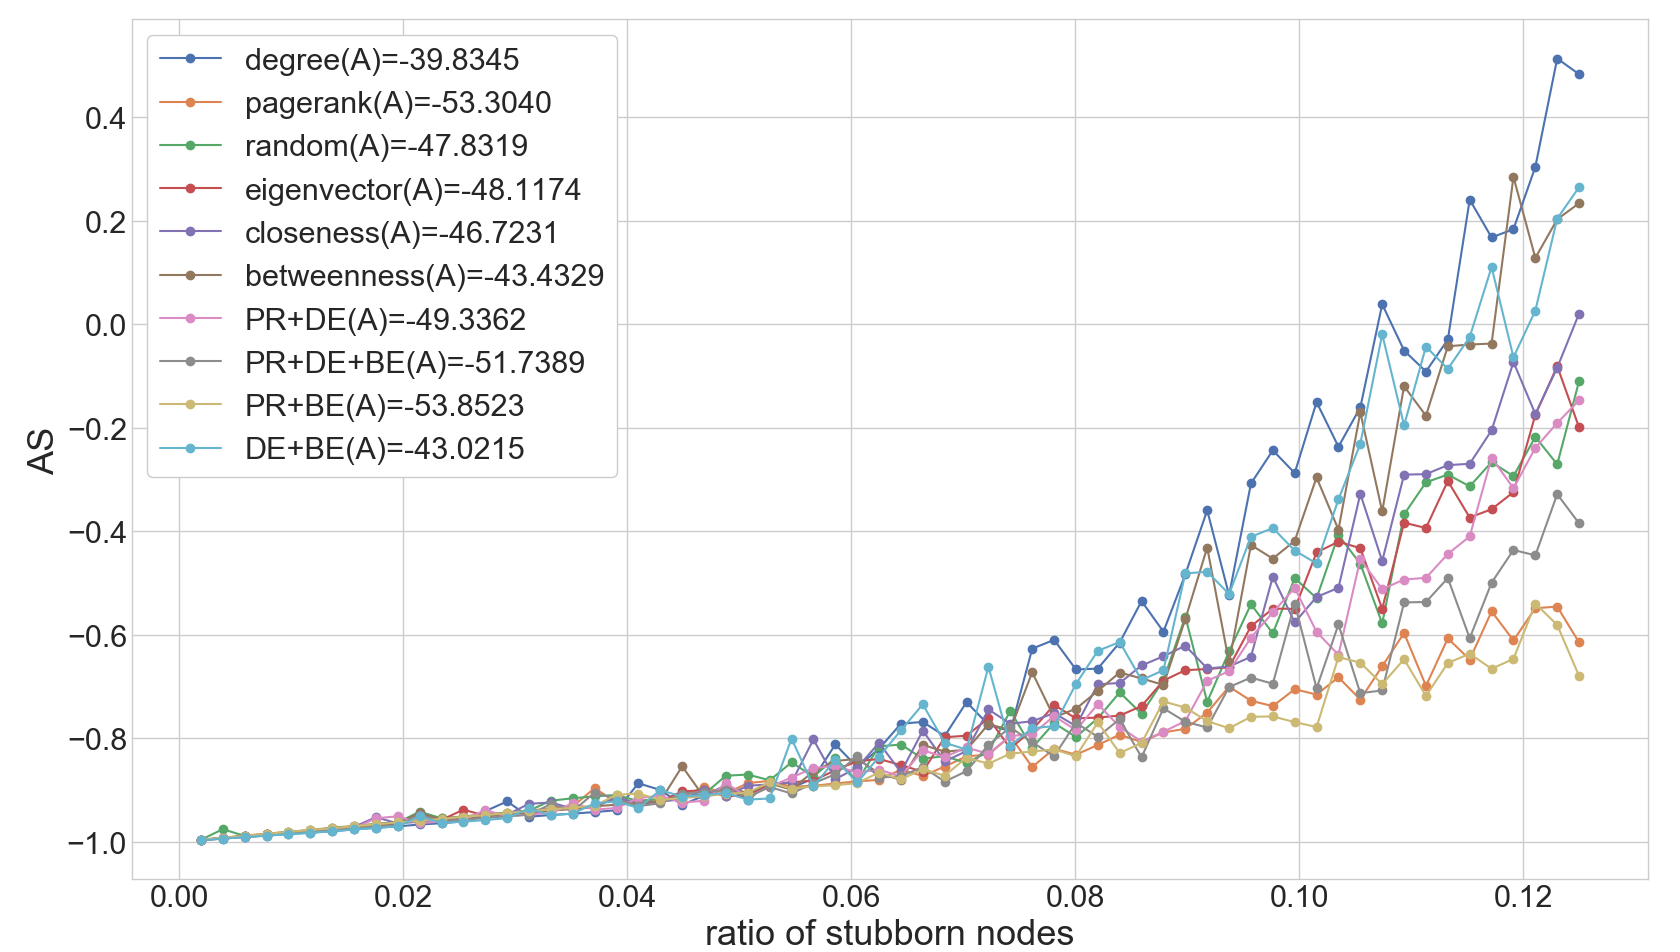
\includegraphics[width=\hsize]{figure/chap5_keynode_RR_BA_A.png}
	\caption{Key nodes on layer A in \textit{RR(6)-BA(3)} network($p=0.2, v=0.4$)}
	\label{chap5_keynode_RR_BA_A}
\end{figure}
\begin{figure}[!htb]
	\centering
	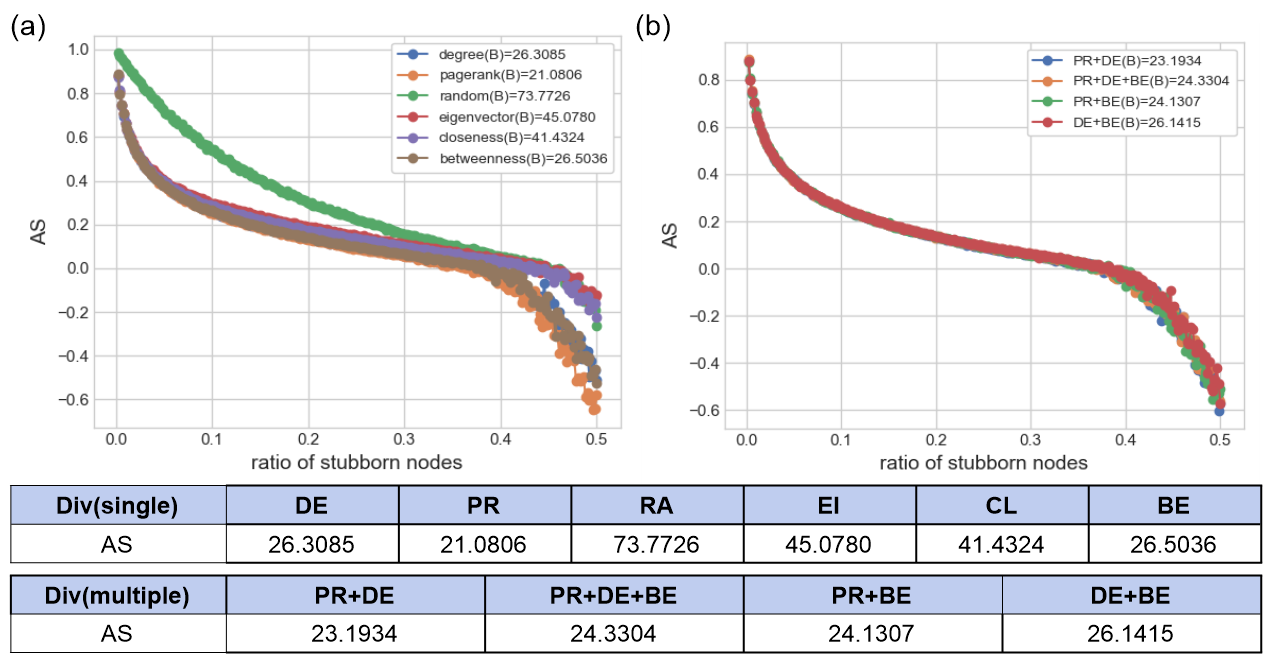
\includegraphics[width=\hsize]{figure/chap5_keynode_RR_BA_B.png}
	\caption{Key nodes on layer B in \textit{RR(6)-BA(3)} network($p=0.3, v=0.5$)}
	\label{chap5_keynode_RR_BA_B}
\end{figure}

Next, the \textit{RR-BA} network is considered. Fig.~\ref{chap5_keynode_RR_BA_A} shows the simulation result of key nodes on layer A. The best method is degree centrality. However, in this model, degree centrality is not meant for recognizing key nodes because all nodes in layer A have the same degree. Here, the reason why degree centrality has an excellent performance in this model is analyzed as follows. Those dynamics are very efficient because nodes are sequentially changed into the stubborn node and interacted (when nodes have the same node centrality, nodes are changed into stubborn nodes sequentially according to interaction order under given algorithm). Other single indicators have similar \textit{AS} values with the random method. The random method has the middle rank. That means node centralities do not work well for identifying key nodes though betweenness has better performance than other methods. Compared with the \textit{BA(3)-BA(3)} shown in Fig.~\ref{chap5_keynode_A}, \textit{RR(6)-BA(3)} has smaller \textit{AS} values and does not reach the opposite consensus yet. 

Fig.~\ref{chap5_keynode_RR_BA_B} shows the simulation result of key nodes on layer B. Pagerank has the best performance. The next rank is \textit{PR+DE}.  Compared with the \textit{BA(3)-BA(3)} shown in Fig.~\ref{chap5_keynode_B} , the \textit{RR(6)-BA(3)} has more massive \textit{AS} values and a more gentle curve to change the state of the network. 

Compared with the \textit{BA-BA} network, both \textit{BA-RR} and \textit{RR-BA} have a more gentle curve line to change the state of the network. It can be analyzed that the \textit{RR} network causes that the critical nodes change the state of the network much more slowly. Moreover, the indexes for key nodes are hard to select critical nodes though betweenness has excellent performance on the \textit{RR} network.\\  

\subsection{Key nodes on the two-layer network with different number of internal links}
Next, the case is considered that each layer has a different number of internal edges. In case that layer A has a more massive number of internal links, layer A consists of a \textit{BA} network with $k=4$, but layer B consists of a \textit{BA} network with $k=2$. Inversely, in case that layer B has a more massive number of internal links, layer B consists of a \textit{BA} network with $k=4$, but layer A consists of a \textit{BA} network with $k=2$. 

\begin{figure}[!htb]
	\centering
	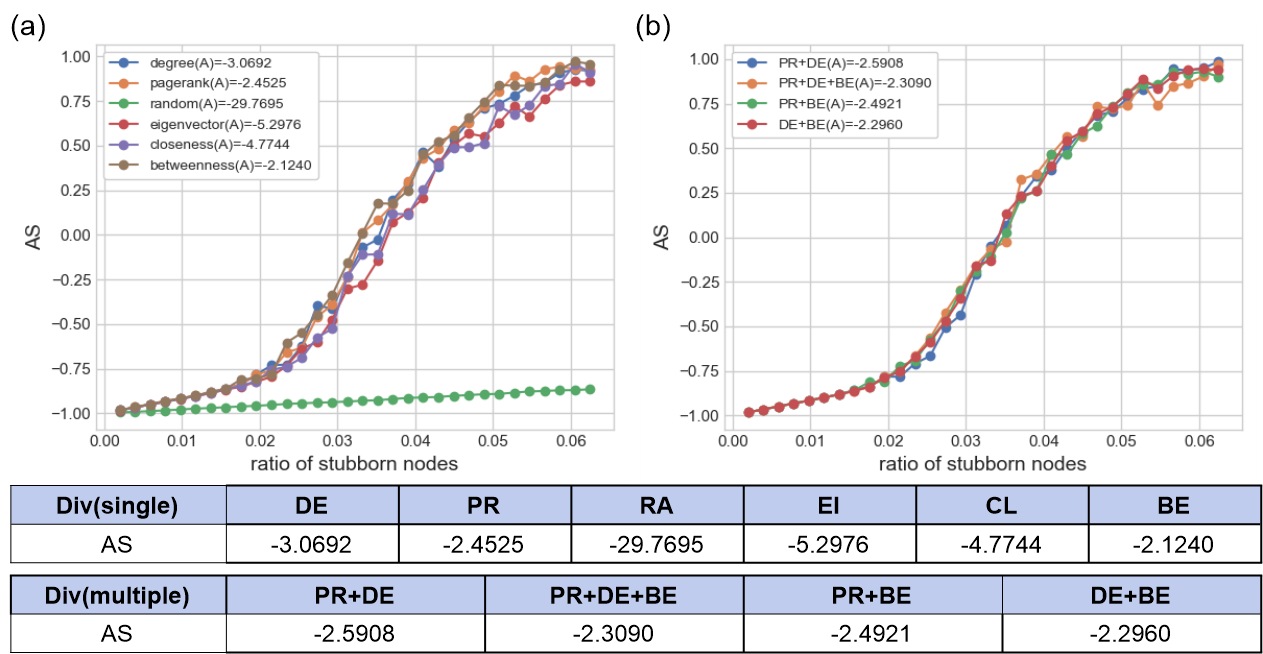
\includegraphics[width=\hsize]{figure/chap5_keynode_internal_A.png}
	\caption{Key nodes on layer A in \textit{BA(4)-BA(2)} network($p=0.15, v=0.3$)}
	\label{chap5_keynode_internal_A}
\end{figure}
\begin{figure}[!htb]
	\centering
	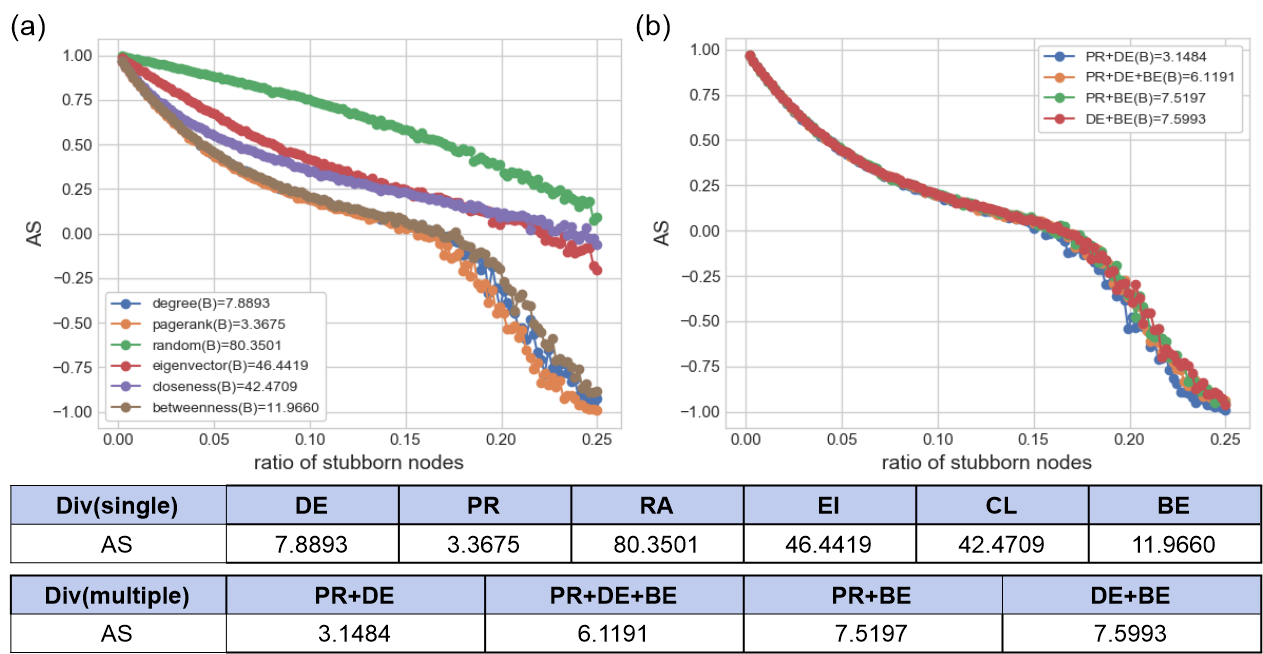
\includegraphics[width=\hsize]{figure/chap5_keynode_internal_B.png}
	\caption{Key nodes on layer B in \textit{BA(4)-BA(2)} network($p=0.2, v=0.4$)}
	\label{chap5_keynode_internal_B}
\end{figure}

First, the case of more internal links on layer A than layer B is investigated. Fig.~\ref{chap5_keynode_internal_A} shows the simulation result of key nodes on layer A in the \textit{BA(4)-BA(2)} network. Betweenness has the best performance for selecting key nodes. The next ranks are \textit{DE+BE}, \textit{PR+BE}, and \textit{PR+DE+BE}. Compared with the \textit{BA(2)-BA(4)} network shown in Fig.~\ref{chap5_keynode_internal_A2}, the curve of changing the state that is shown in Fig.~\ref{chap5_keynode_internal_A} is much more straight-line. That means consensus time is short, and key nodes make a consensus much quickly.

Fig.~\ref{chap5_keynode_internal_B} shows the simulation result of key nodes on layer B in the \textit{BA(4)-BA(2)} network. \textit{PR+DE} is the most powerful method. The next ranks are Pagerank, \textit{PR+DE+BE}, and \textit{PR+BE}. Compared with the \textit{BA(2)-BA(4)} network shown in Fig.~\ref{chap5_keynode_internal_B2}, the curve of changing the state that is shown in Fig.~\ref{chap5_keynode_internal_B} is also more straight-line. 

Compared with the \textit{BA(2)-BA(4)} network, it can be analyzed that more internal edges on layer A effect that key nodes make a consensus much quickly. 

\begin{figure}[!htb]
	\centering
	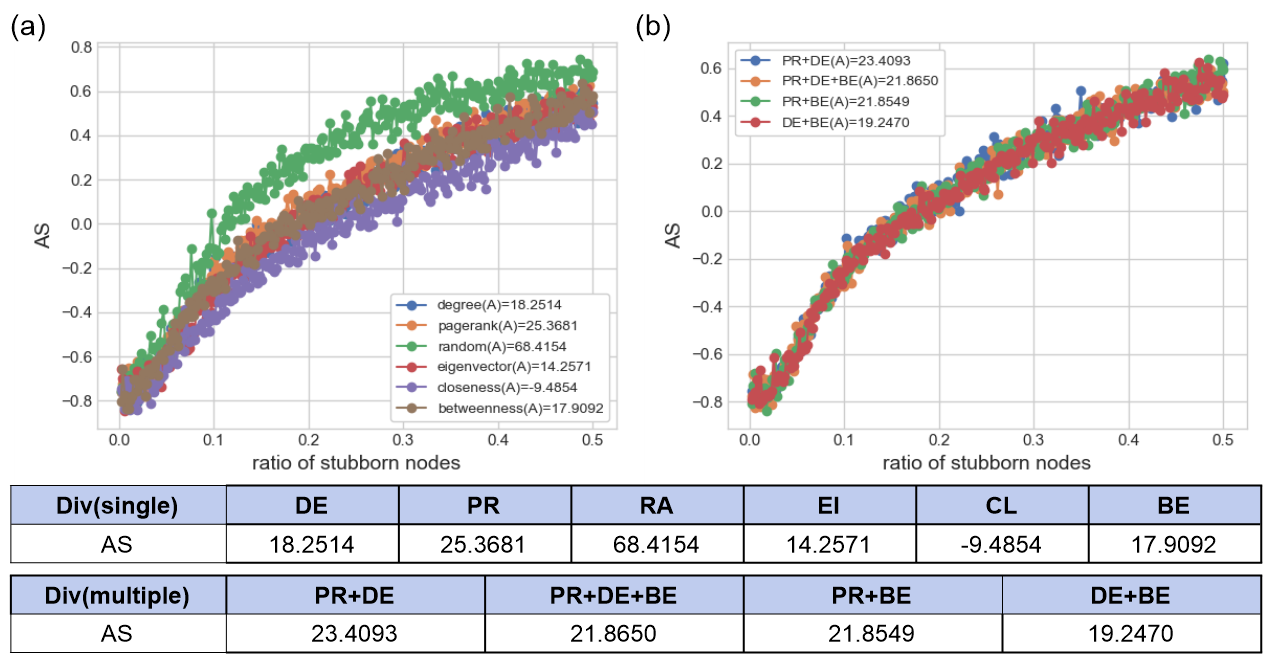
\includegraphics[width=\hsize]{figure/chap5_keynode_internal_A2.png}
	\caption{Key nodes on layer A in \textit{BA(2)-BA(4)} network($p=0.57, v=0.37$)}
	\label{chap5_keynode_internal_A2}
\end{figure}
\begin{figure}[!htb]
	\centering
	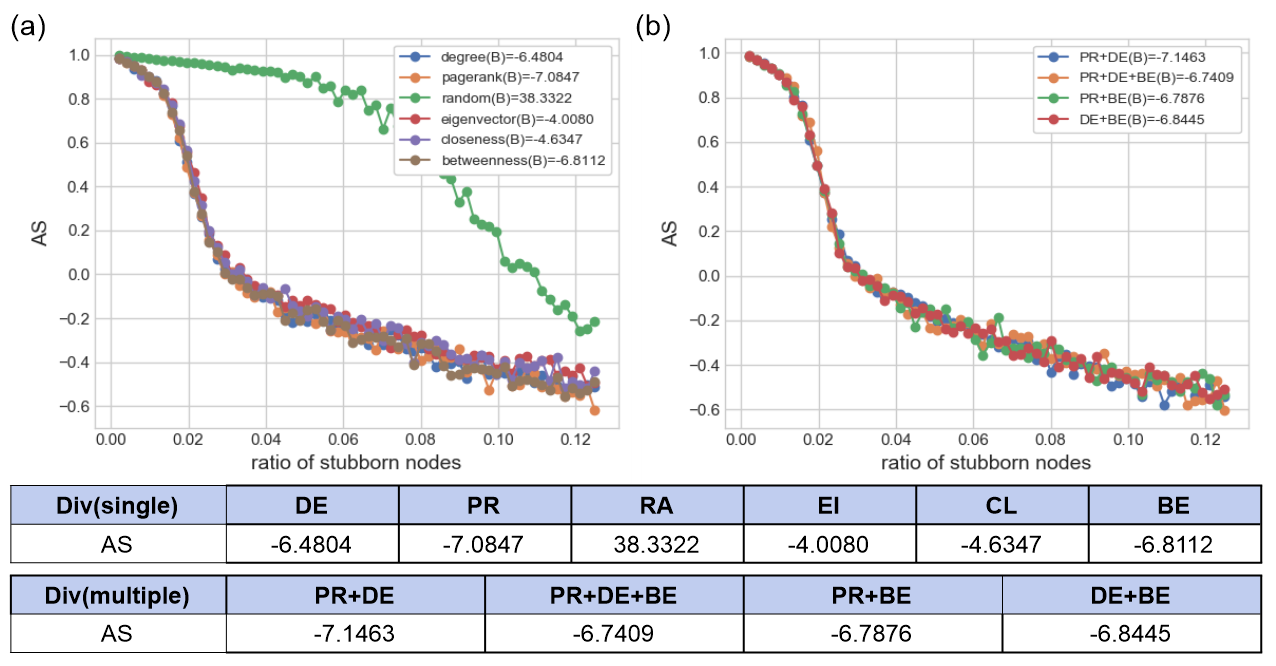
\includegraphics[width=\hsize]{figure/chap5_keynode_internal_B2.png}
	\caption{Key nodes on layer B in \textit{BA(2)-BA(4)} network($p=0.6, v=0.4$)}
	\label{chap5_keynode_internal_B2}
\end{figure}

Next, the case of more internal links on layer B than layer A is researched. Fig.~\ref{chap5_keynode_internal_A2} shows the simulation result of key nodes on layer A in the \textit{BA(2)-BA(4)} network. However, the simulation results are different from other results because the random method has the best performance. That means node centralities do not work on this model. Compared with the \textit{BA(4)-BA(2)} network shown in Fig.~\ref{chap5_keynode_internal_A}, the curve of changing the state that is shown in Fig.~\ref{chap5_keynode_internal_A2}  is much slower and more gentle.

Fig.~\ref{chap5_keynode_internal_B2} shows the simulation result of key nodes on layer B in the \textit{BA(2)-BA(4)} network. \textit{PR+DE} has the most effective performance. The next ranks are Pagerank, \textit{DE+BE}, and betweenness. Compared with the \textit{BA(4)-BA(2)} network shown in Fig.~\ref{chap5_keynode_internal_B}, the curve of changing the state that is shown in Fig.~\ref{chap5_keynode_internal_B2} is much faster at the beginning but much slower at the end. Besides, consensus does not happen in this model.

Compared with the \textit{BA(4)-BA(2)} network, it can be analyzed that the larger number of internal edges on layer B causes that key nodes make consensus much harder. Moreover, decreasing internal edges on layer A effects that the indexes for key nodes are hard to select critical nodes on layer A.\\   

\section{Conclusion}
By using node centrality and combined node centrality, key nodes on each layer have been recognized on networks with various structures. Table~\ref{effective methods} shows the total simulation results for selecting key nodes on various interconnected networks.
 
\begin{table}[!htb]
	\scriptsize
	\centering
	\caption{Effective method for selecting key nodes on various networks}
	\label{effective methods}
	\begin{center}
		\begin{tabular}{c|c|c|c|c|c|c|c|c|c} \hline\hline
		  Div                              & A nodes & B nodes & A edges & B edges & layer & 1st method & 2nd method  & 3rd method  & remarks    \\ \hline \hline
         \multirow{1}{*}{BA(3)-BA(3)}      & 512 	 & 512     & 1,527   & 1,527   & A     & PR+BE      & PR+DE       & Pagerank    &            \\ 
			                               &  	     &         &         &         & B     & Pagerank   & PR+DE       & PR+BE       &		     \\ \hline   
	     \multirow{1}{*}{BA(3)-RR(6)}      & 512     & 512     & 1,527   & 1,536   & A     & PR+BE      & Pagerank    & PR+DE+BE    &            \\
	                                       &         &         &         &         & B     & betweenness& DE+BE       & random      & not working\\ \hline
	     \multirow{1}{*}{RR(6)-BA(3)}      & 512     & 512     & 1,536   & 1,527   & A     & degree     & DE+BE       & betweenness & not working\\ 
	                                       &         &         &         &         & B     & Pagerank   & PR+DE       & PR+BE       &            \\ \hline
		 \multirow{1}{*}{BA(4)-BA(2)}      & 512     & 512     & 2,032   & 1,020   & A     & betweenness& DE+BE       & PR+BE       &            \\ 
		                                   &         &         &         &         & B     & PR+DE      & Pagerank    & PR+DE+BE    &            \\ \hline
		 \multirow{1}{*}{BA(2)-BA(4)}      & 512     & 512     & 1,020   & 2,032   & A     & random     & Pagerank    & PR+DE       & not working\\ 
		                                   &         &         &         &         & B     & PR+DE      & Pagerank    & DE+BE       &            \\ \hline
		 \multirow{1}{*}{HM(8) with BA(3)} & 512     & 64      & 1,527   & 183     & A     & PR+DE      & PR+BE       & Pagerank    &            \\ 
		                                   &         &         &         &         & B     & random     & DE+BE       & PR+DE+BE    & not working\\ \hline
			\hline
		\end{tabular}
	\end{center}
\end{table}

Here, we find several facts from these simulation results. First, it can be found out that the best and most powerful method for selecting key nodes is different according to network structures and layers. Second, as single indicators, Pagerank, degree, and betweenness are an excellent method to select key nodes on a two-layer network. Third, as multiple indicators, combined node centralities have an excellent performance to recognize the critical nodes on various networks. Combined node centralities are the first or second effective methods of all simulation models.(except not working methods) Fourth, as shown in interconnected networks with a different internal degree on each layer, a larger degree on layer A effects that key nodes make a consensus much easily. Otherwise, a larger degree on layer B causes that key nodes make a consensus much harder. Besides, a decrease of an internal degree in layer A produces that the indexes for selecting key nodes are hard to recognize key nodes on layer A. Fifth, as shown in the \textit{HM(8) with BA(3)} network, that is modeled by decreasing nodes in layer B and increasing the external degree in layer B,  the \textit{Hierarchical Model} causes that the indexes for recognizing key nodes are hard to identify critical nodes on layer B.  Moreover, the \textit{Hierarchical Model} is easy to reach consensus by key nodes. Sixth, as shown in interconnected networks with different network types, network types influence whether a network can make consensus by key nodes or not. Notably, it is shown that the \textit{RR} network makes it slow to have a consensus by key nodes, and effects that the indexes for selecting key nodes are hard to recognize critical nodes. Through these simulations, it can provide some preliminary results, such as how to choose the leader, and how to intervene the social opinion through key nodes. Considering the structures and layers of networks, node centralities or combined node centralities can be used to recognize the leaders or the key agents.\\
